\documentclass{standalone}
\usepackage{tikz}
\usetikzlibrary{patterns, positioning}


\begin{document}
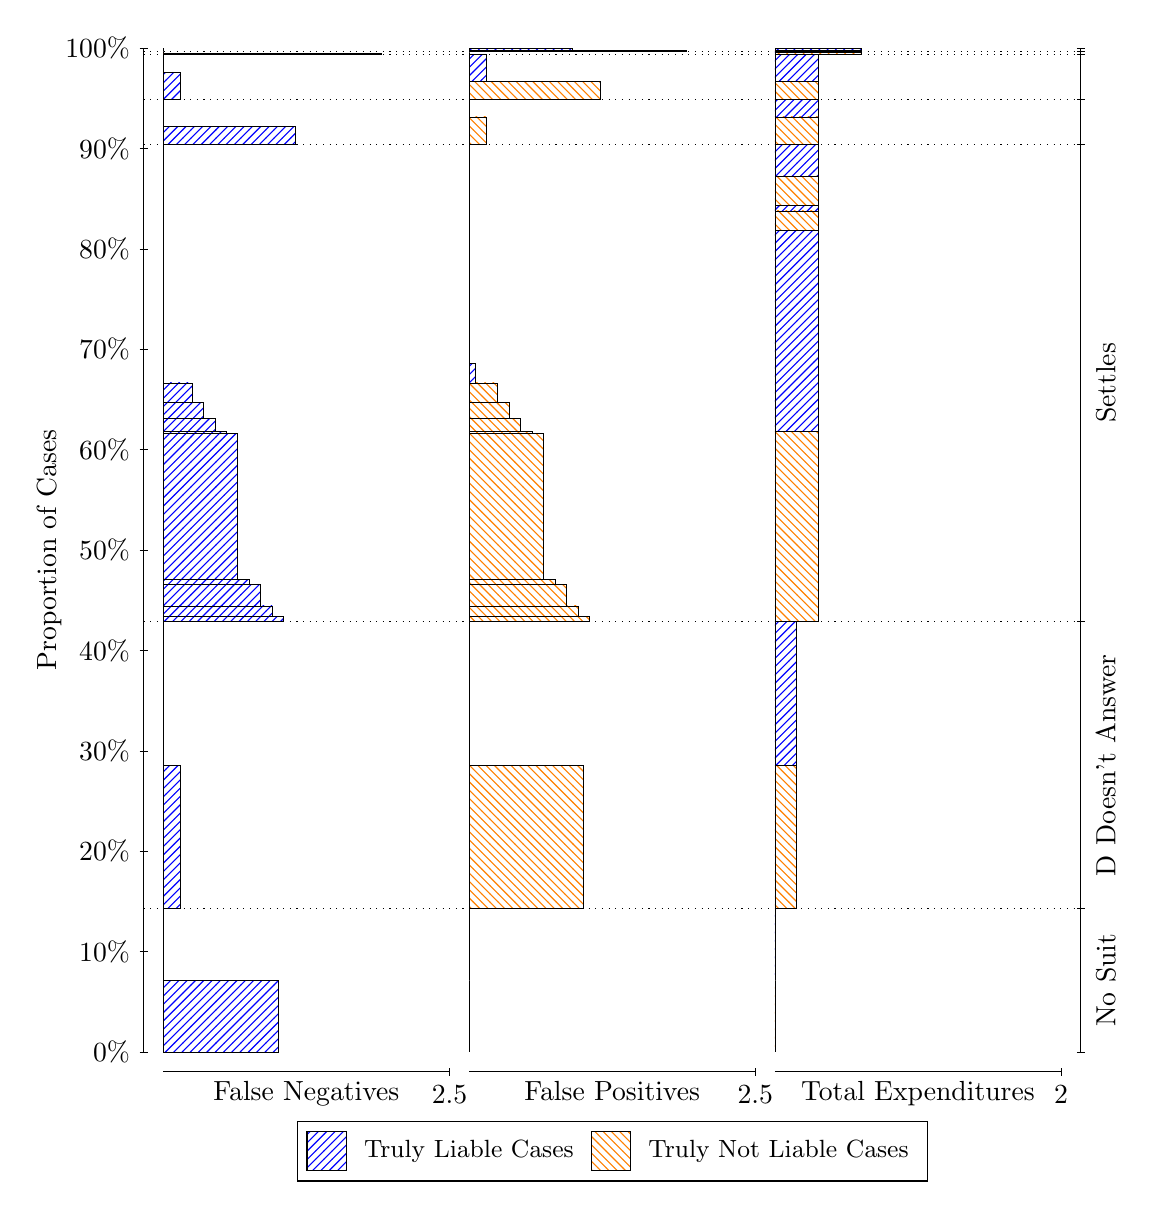
\begin{tikzpicture}
\draw[black, very thin] (1.5,1.75) -- (1.5,14.5);
\node[rotate=90, text=black, anchor=center] at (0.3, 8.125) {Proportion of Cases};
\draw[black, very thin] (1.45,1.75) -- (1.55,1.75);
\node[text=black, anchor=east] at (1.45, 1.75) {0\%};
\draw[black, very thin] (1.45,3.025) -- (1.55,3.025);
\node[text=black, anchor=east] at (1.45, 3.025) {10\%};
\draw[black, very thin] (1.45,4.3) -- (1.55,4.3);
\node[text=black, anchor=east] at (1.45, 4.3) {20\%};
\draw[black, very thin] (1.45,5.575) -- (1.55,5.575);
\node[text=black, anchor=east] at (1.45, 5.575) {30\%};
\draw[black, very thin] (1.45,6.85) -- (1.55,6.85);
\node[text=black, anchor=east] at (1.45, 6.85) {40\%};
\draw[black, very thin] (1.45,8.125) -- (1.55,8.125);
\node[text=black, anchor=east] at (1.45, 8.125) {50\%};
\draw[black, very thin] (1.45,9.4) -- (1.55,9.4);
\node[text=black, anchor=east] at (1.45, 9.4) {60\%};
\draw[black, very thin] (1.45,10.675) -- (1.55,10.675);
\node[text=black, anchor=east] at (1.45, 10.675) {70\%};
\draw[black, very thin] (1.45,11.95) -- (1.55,11.95);
\node[text=black, anchor=east] at (1.45, 11.95) {80\%};
\draw[black, very thin] (1.45,13.225) -- (1.55,13.225);
\node[text=black, anchor=east] at (1.45, 13.225) {90\%};
\draw[black, very thin] (1.45,14.5) -- (1.55,14.5);
\node[text=black, anchor=east] at (1.45, 14.5) {100\%};

\draw[black, very thin] (13.4,1.75) -- (13.4,14.5);
\draw[black, very thin] (13.35,1.75) -- (13.45,1.75);
\node[anchor=west] at (13.35, 1.75) {};
\draw[black, very thin] (13.35,3.5714) -- (13.45,3.5714);
\node[anchor=west] at (13.35, 3.5714) {};
\draw[black, very thin] (13.35,7.2143) -- (13.45,7.2143);
\node[anchor=west] at (13.35, 7.2143) {};
\draw[black, very thin] (13.35,13.28) -- (13.45,13.28);
\node[anchor=west] at (13.35, 13.28) {};
\draw[black, very thin] (13.35,13.849) -- (13.45,13.849);
\node[anchor=west] at (13.35, 13.849) {};
\draw[black, very thin] (13.35,14.417) -- (13.45,14.417);
\node[anchor=west] at (13.35, 14.417) {};
\draw[black, very thin] (13.35,14.459) -- (13.45,14.459);
\node[anchor=west] at (13.35, 14.459) {};
\draw[black, very thin] (13.35,14.5) -- (13.45,14.5);
\node[anchor=west] at (13.35, 14.5) {};

\draw[black, very thin, pattern color=blue, pattern=north east lines] (1.75,1.75) rectangle (3.2033,2.6607);
\draw[black, very thin, pattern color=orange, pattern=north west lines] (1.75,2.6607) rectangle (1.75,3.5714);
\draw[black, very thin, pattern color=blue, pattern=north east lines] (1.75,3.5714) rectangle (1.968,5.3929);
\draw[black, very thin, pattern color=orange, pattern=north west lines] (1.75,5.3929) rectangle (1.75,7.2143);
\draw[black, very thin, pattern color=blue, pattern=north east lines] (1.75,7.2143) rectangle (3.276,7.2811);
\draw[black, very thin, pattern color=blue, pattern=north east lines] (1.75,7.2811) rectangle (3.1307,7.4164);
\draw[black, very thin, pattern color=blue, pattern=north east lines] (1.75,7.4164) rectangle (2.9853,7.6864);
\draw[black, very thin, pattern color=blue, pattern=north east lines] (1.75,7.6864) rectangle (2.84,7.7492);
\draw[black, very thin, pattern color=blue, pattern=north east lines] (1.75,7.7492) rectangle (2.6947,9.6058);
\draw[black, very thin, pattern color=blue, pattern=north east lines] (1.75,9.6058) rectangle (2.5493,9.6266);
\draw[black, very thin, pattern color=blue, pattern=north east lines] (1.75,9.6266) rectangle (2.404,9.7993);
\draw[black, very thin, pattern color=blue, pattern=north east lines] (1.75,9.7993) rectangle (2.2587,10.003);
\draw[black, very thin, pattern color=blue, pattern=north east lines] (1.75,10.003) rectangle (2.1133,10.247);
\draw[black, very thin, pattern color=orange, pattern=north west lines] (1.75,10.247) rectangle (1.75,13.28);
\draw[black, very thin, pattern color=blue, pattern=north east lines] (1.75,13.28) rectangle (3.4213,13.503);
\draw[black, very thin, pattern color=orange, pattern=north west lines] (1.75,13.503) rectangle (1.75,13.849);
\draw[black, very thin, pattern color=blue, pattern=north east lines] (1.75,13.849) rectangle (1.968,14.194);
\draw[black, very thin, pattern color=orange, pattern=north west lines] (1.75,14.194) rectangle (1.75,14.417);
\draw[black, very thin, pattern color=blue, pattern=north east lines] (1.75,14.417) rectangle (4.5113,14.433);
\draw[black, very thin, pattern color=orange, pattern=north west lines] (1.75,14.433) rectangle (1.75,14.459);
\draw[black, very thin, pattern color=orange, pattern=north west lines] (1.75,14.459) rectangle (1.75,14.474);
\draw[black, very thin, pattern color=blue, pattern=north east lines] (1.75,14.474) rectangle (1.75,14.5);
\draw[black, very thin, pattern color=orange, pattern=north west lines] (5.6333,1.75) rectangle (5.6333,2.6607);
\draw[black, very thin, pattern color=blue, pattern=north east lines] (5.6333,2.6607) rectangle (5.6333,3.5714);
\draw[black, very thin, pattern color=orange, pattern=north west lines] (5.6333,3.5714) rectangle (7.0867,5.3929);
\draw[black, very thin, pattern color=blue, pattern=north east lines] (5.6333,5.3929) rectangle (5.6333,7.2143);
\draw[black, very thin, pattern color=orange, pattern=north west lines] (5.6333,7.2143) rectangle (7.1593,7.2811);
\draw[black, very thin, pattern color=orange, pattern=north west lines] (5.6333,7.2811) rectangle (7.014,7.4164);
\draw[black, very thin, pattern color=orange, pattern=north west lines] (5.6333,7.4164) rectangle (6.8687,7.6864);
\draw[black, very thin, pattern color=orange, pattern=north west lines] (5.6333,7.6864) rectangle (6.7233,7.7492);
\draw[black, very thin, pattern color=orange, pattern=north west lines] (5.6333,7.7492) rectangle (6.578,9.6058);
\draw[black, very thin, pattern color=orange, pattern=north west lines] (5.6333,9.6058) rectangle (6.4327,9.6266);
\draw[black, very thin, pattern color=orange, pattern=north west lines] (5.6333,9.6266) rectangle (6.2873,9.7993);
\draw[black, very thin, pattern color=orange, pattern=north west lines] (5.6333,9.7993) rectangle (6.142,10.003);
\draw[black, very thin, pattern color=orange, pattern=north west lines] (5.6333,10.003) rectangle (5.9967,10.247);
\draw[black, very thin, pattern color=blue, pattern=north east lines] (5.6333,10.247) rectangle (5.706,10.491);
\draw[black, very thin, pattern color=blue, pattern=north east lines] (5.6333,10.491) rectangle (5.6333,13.28);
\draw[black, very thin, pattern color=orange, pattern=north west lines] (5.6333,13.28) rectangle (5.8513,13.625);
\draw[black, very thin, pattern color=blue, pattern=north east lines] (5.6333,13.625) rectangle (5.6333,13.849);
\draw[black, very thin, pattern color=orange, pattern=north west lines] (5.6333,13.849) rectangle (7.3047,14.072);
\draw[black, very thin, pattern color=blue, pattern=north east lines] (5.6333,14.072) rectangle (5.8513,14.417);
\draw[black, very thin, pattern color=orange, pattern=north west lines] (5.6333,14.417) rectangle (5.6333,14.443);
\draw[black, very thin, pattern color=blue, pattern=north east lines] (5.6333,14.443) rectangle (5.6333,14.459);
\draw[black, very thin, pattern color=orange, pattern=north west lines] (5.6333,14.459) rectangle (8.3947,14.474);
\draw[black, very thin, pattern color=blue, pattern=north east lines] (5.6333,14.474) rectangle (6.9413,14.5);
\draw[black, very thin, pattern color=orange, pattern=north west lines] (9.5167,1.75) rectangle (9.5167,2.6607);
\draw[black, very thin, pattern color=blue, pattern=north east lines] (9.5167,2.6607) rectangle (9.5167,3.5714);
\draw[black, very thin, pattern color=orange, pattern=north west lines] (9.5167,3.5714) rectangle (9.7892,5.3929);
\draw[black, very thin, pattern color=blue, pattern=north east lines] (9.5167,5.3929) rectangle (9.7892,7.2143);
\draw[black, very thin, pattern color=orange, pattern=north west lines] (9.5167,7.2143) rectangle (10.062,9.6266);
\draw[black, very thin, pattern color=blue, pattern=north east lines] (9.5167,9.6266) rectangle (10.062,12.187);
\draw[black, very thin, pattern color=orange, pattern=north west lines] (9.5167,12.187) rectangle (10.062,12.431);
\draw[black, very thin, pattern color=blue, pattern=north east lines] (9.5167,12.431) rectangle (10.062,12.498);
\draw[black, very thin, pattern color=orange, pattern=north west lines] (9.5167,12.498) rectangle (10.062,12.875);
\draw[black, very thin, pattern color=blue, pattern=north east lines] (9.5167,12.875) rectangle (10.062,13.28);
\draw[black, very thin, pattern color=orange, pattern=north west lines] (9.5167,13.28) rectangle (10.062,13.625);
\draw[black, very thin, pattern color=blue, pattern=north east lines] (9.5167,13.625) rectangle (10.062,13.849);
\draw[black, very thin, pattern color=orange, pattern=north west lines] (9.5167,13.849) rectangle (10.062,14.072);
\draw[black, very thin, pattern color=blue, pattern=north east lines] (9.5167,14.072) rectangle (10.062,14.417);
\draw[black, very thin, pattern color=orange, pattern=north west lines] (9.5167,14.417) rectangle (10.607,14.443);
\draw[black, very thin, pattern color=blue, pattern=north east lines] (9.5167,14.443) rectangle (10.607,14.459);
\draw[black, very thin, pattern color=orange, pattern=north west lines] (9.5167,14.459) rectangle (10.607,14.474);
\draw[black, very thin, pattern color=blue, pattern=north east lines] (9.5167,14.474) rectangle (10.607,14.5);
\draw[black, dotted] (1.5,3.5714) -- (13.4,3.5714);
\draw[black, dotted] (1.5,7.2143) -- (13.4,7.2143);
\draw[black, dotted] (1.5,13.28) -- (13.4,13.28);
\draw[black, dotted] (1.5,13.849) -- (13.4,13.849);
\draw[black, dotted] (1.5,14.417) -- (13.4,14.417);
\draw[black, dotted] (1.5,14.459) -- (13.4,14.459);
\draw[black, very thin] (1.75,1.5) -- (5.3833,1.5);
\node[text=black, anchor=north] at (3.5667, 1.5) {False Negatives};
\draw[black, very thin] (5.3833,1.45) -- (5.3833,1.55);
\node[text=black, anchor=north] at (5.3833, 1.45) {2.5};

\draw[black, very thin] (5.6333,1.5) -- (9.2667,1.5);
\node[text=black, anchor=north] at (7.45, 1.5) {False Positives};
\draw[black, very thin] (9.2667,1.45) -- (9.2667,1.55);
\node[text=black, anchor=north] at (9.2667, 1.45) {2.5};

\draw[black, very thin] (9.5167,1.5) -- (13.15,1.5);
\node[text=black, anchor=north] at (11.333, 1.5) {Total Expenditures};
\draw[black, very thin] (13.15,1.45) -- (13.15,1.55);
\node[text=black, anchor=north] at (13.15, 1.45) {2};

\node[text=black, centered, rotate=90] at (13.72, 2.6607) {No Suit};
\node[text=black, centered, rotate=90] at (13.72, 5.3929) {D Doesn't Answer};
\node[text=black, centered, rotate=90] at (13.72, 10.247) {Settles};





\draw (7.449999999999999,1.5) node[draw=none] (baseCoordinate) {};
\begin{scope}[align=center]
        \matrix[scale=0.5, draw=black, below=0.5cm of baseCoordinate, nodes={draw}, column sep=0.1cm]{
            \node[rectangle, draw, minimum width=0.5cm, minimum height=0.5cm, pattern color=blue, pattern=north east lines] {}; &
            \node[draw=none, font=\small, text=black] (B) {Truly Liable Cases}; &
            \node[rectangle, draw, minimum width=0.5cm, minimum height=0.5cm, pattern color=orange, pattern=north west lines] {}; &
            \node[draw=none, font=\small, text=black] (B) {Truly Not Liable Cases}; \\
            };
\end{scope}

\end{tikzpicture}
\end{document}